\chapter{TECNOLOGIAS EMPREGADAS}

Este capitulo faz uma introdução das tecnologias utilizadas, tais como o Samba, NetBIOS, \textit{Active Directory}, DNS, LDAP, Kerberos, entre outros, além da apresentação de termos técnicos essenciais para o melhor entendimento deste trabalho.

\section{Samba}

Samba é um \textit{software} \textit{open source} que provê serviços a clientes utilizando os protocolos SMB e CIFS.
O samba permite a interoperabilidade entre servidores Linux/Unix e clientes baseados na
plataforma Windows.
O samba permite que um servidor Linux seja apto a fornecer serviços como:
  \begin{itemize}
    \item \textbf{Servidor de arquivos e impressão} - Utilizando o protocolo \textit{Server Message Block} para possibilitar o compartilhamento de arquivos, pastas volumes e impressoras na rede, com um controle de permissões de acessos a usuários e grupos juntamente com as permissões locais atribuídas as pastas compartilhadas. Algumas permissões de acesso local serão explicadas no tópico sobre permissões especiais no Linux.

    \item \textbf{Autenticação e autorização} - Identifica um computador ou um usuário da rede e determina os direitos de acesso a arquivos que cada usuário possui, através de tecnologias como permissões de arquivos, diretivas de grupo e o serviço de autenticação Kerberos.

    \item \textbf{Resolução e busca de nomes e diretórios} - Compartilha as principais informações sobre computadores e usuários da rede através do \textit{LightWeight Directory Access Protocol} (LDAP).% e o Microsoft Active Directory.

    \item \textbf{Servidor de domínio como PDC} - Funcionando como controlador de domínio ativo dentro de um domínio Windows. Para melhor entendimento ele será explicado no tópico sobre PDC.
  \end{itemize}

Basicamente, o Samba é um servidor e um conjunto de ferramentas que permite o compartilhamento de arquivos e impressoras em sistemas Windows e Linux. Outra característica do Samba é poder atuar como um Controlador Primário de Domínio (PDC), armazenando perfis de usuários e realizar controle de acesso. \cite{FOCA}.

\section{PDC}

O Controlador de Domínio é responsável por fornecer autenticação para os clientes, sejam sistemas Linux ou Windows. Ou seja, apenas centraliza contas de usuários e fornece recursos voltados para a administração de usuários, como a gestão de perfis móveis, que são as configurações de usuários que são lidas, independente de qual máquina o usuário utilize. Em uma rede com mais de 10 clientes a necessidade de ter um PDC é mais aparente, pois fica cada vez mais difícil gerenciar as contas de clientes e máquinas conforme o crescimento da mesma. Com o Controlador de Domínio também é possível fornecer acesso por perfis móveis onde o usuário pode ter acesso à sua área de trabalho independente da máquina (da mesma rede) onde faz o login. Em contrapartida, bloqueando uma conta de usuário,automaticamente este estará bloqueado em todas as máquinas gerenciadas pelo Controlador de Domínio \cite{MORIMOTO}

\section{Permissões especiais no Linux}

Existe no Linux três permissões especiais, para dar segurança ao sistema, chamadas assim por somente serem atribuídas a arquivos específicos (arquivos executáveis e diretórios). Tais permissões são fornecidas pelos bits SUID, SGID e STICKY.

  \begin{itemize}
    \item \textbf{SUID} - O bit SUID (Set UID) é aplicável apenas a arquivos executáveis, fazendo com que estes rodem com as permissões de seu proprietário, independente de quem tenha executado-o. Pode ser útil para que usuários comuns possam executar arquivos permitidos apenas a administradores.

    \item \textbf{SGID} - O bit SGID (Set GID) pode ser aplicado a um arquivo executável e a um diretório. No primeiro caso ele tem as mesma função do SUID, porém rodando com as permissões de um grupo de usuários. No segundo, ele força os arquivos e diretórios criados dentro do diretório pai (o que obteve a permissão) a pertencerem ao mesmo grupo, independente do grupo de quem o tenha criado.

    \item \textbf{STICKY} - O bit STICKY é aplicável a diretórios e faz com que a exclusão de arquivos pertencentes a estes diretórios seja apenas permitida ao dono do arquivo e ao administrador do sistema. Tem vantagem sobre a permissão “Somente Leitura” no diretório pois faz com que outros usuários possam criar e editar qualquer arquivo, impedindo-os apenas de apagá-lo.
  \end{itemize}

É importante ressaltar que de nada adiantará se os arquivos e diretórios possuírem determinadas permissões locais se as concedidas através do Samba não forem compatíveis às permissões atribuídas. Por exemplo: de nada adiantará atribuir acesso de escrita a um arquivo no Linux se ele possui permissão ``Somente Leitura" no Samba. A atribuição mais negativa, ou seja, a que concede menos permissões (neste caso a ``Somente Leitura") prevalecerá sobre a outra.

\section{NETBIOS}

Um nome NetBIOS é um endereço de 16 bytes usado para identificar um recurso NetBIOS na rede. Um nome NetBIOS é um nome único (exclusivo) ou de grupo (não exclusivo). Quando um processo de NetBIOS está comunicando-se com um processo específico em um computador específico, é usado um nome exclusivo. Quando um processo de NetBIOS está comunicando-se com vários processos em vários computadores, é usado um nome de grupo. A resolução de nomes NetBIOS significa o mapeamento bem-sucedido de um nome NetBIOS para um endereço IP.\cite{NETBIOS}

O NetBIOS trabalha na camada sessão do modelo OSI (\textit{Open Systems Interconnection}), e utiliza as portas de comunicação UDP (\textit{User Datagram Protocol}) 137 e 138 para a resolução dos NetBios \textit{names} e \textit{datagrams} e 139 de comunicação TCP (\textit{Transmission Control Protocol}) para NetBios \textit{sessions}, conforme a Figura \ref{netbios}

\begin{figure}[ht]
   	\centering
    \scalebox{1}{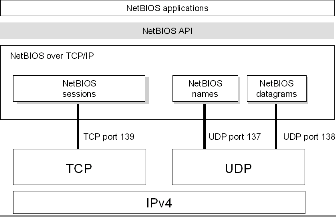
\includegraphics{figuras/netbios}}
   	\caption{Estrutura do funcionamento da NetBios \cite{NETBIOS}}
    \label{netbios}
\end{figure}

\section{\textit{Active Directory}}

O \textit{Active Directory} (AD) é um serviço de diretório nas redes a partir do Windows 2000.

Serviço de diretório é um conjunto de atributos sobre recursos e serviços existentes na rede, isso significa que é uma maneira de organizar e simplificar o acesso aos recursos da rede, centralizando-os; bem como, reforçar a segurança e dar proteção aos objetos da base de dados contra intrusos, ou controlar acessos dos usuários internos da rede.

O \textit{Active Directory} mantém dados como contas de usuários, impressoras, grupos, computadores, servidores, recursos de rede, etc. Ele pode ser totalmente escalonável, aumentando conforme a necessidade.\cite{LOSANO}

\section{LDAP}

O LDAP (\textit{Lightweight Directory Access Protocol}) é o protocolo responsável por fornecer Serviço de Diretórios a computadores Windows de forma similar ao \textit{Active Directory} da Microsoft, que é baseado no LDAP. Tais serviços incluem conexões de computadores, grupos de computadores, usuários, administração de identidades, além de possibilitar uma maneira eficiente de descrever, localizar e administrar esses recursos. Essa estrutura do LDAP pode ser vista na Figura \ref{ldap}

LDAP é um protocolo para acessar informações contidas em um diretório. Por ser um protocolo cliente/servidor o LDAP permite navegar, ler, armazenar e pesquisar informações e realizar tarefas de gerenciamento em um serviço de diretórios. O serviço de diretório é um banco de dados otimizado para leitura, navegação e pesquisas \cite{TRIGO}.

\begin{figure}[ht]
   	\centering
    \scalebox{1}{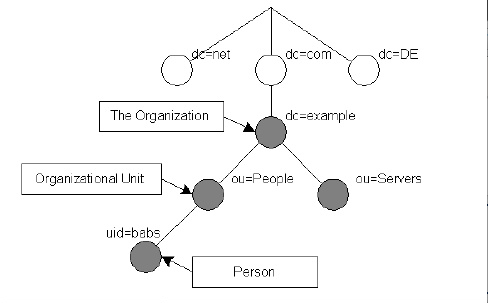
\includegraphics{figuras/ldap}}
   	\caption{Estrutura do protocolo LDAP \cite{LDAP}}
    \label{ldap}
\end{figure}

\section{DNS}

DNS (\textit{Domain Name System}) é uma base de dados hierárquica e distribuída, usada para a resolução de nomes de domínios em endereços IP (\textit{ Internet Protocol}). É considerado como um banco de dados distribuído que converte nomes de \textit{hosts} (máquinas) para endereços IP. É basicamente um mapeamento de endereços IP e seus respectivos nomes. A utilização mais comum é na internet. Todos os computadores da rede possuem um endereço IP. Os servidores DNS simplesmente transformam ou resolvem esse número em um nome \cite{SCRIMER}. Por exemplo, o endereço www.iff.edu.br corresponde ao IP 200.143.198.110. Exemplos de domínios DNS que podem ser visto na Figura \ref{dns}

\begin{figure}[ht]
   	\centering
    \scalebox{1}{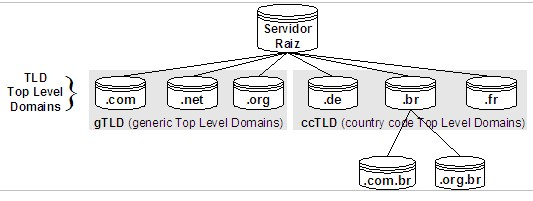
\includegraphics{figuras/servidor_dns}}
   	\caption{Estrutura hierárquica do DNS \cite{DNS}}
    \label{dns}
\end{figure}

\section{BIND}

BIND é um \textit{software} de código livre que implementa o Sistema de Nomes de Domínio (DNS) de protocolos para a internet. É uma referência em implementação desses protocolos, mas também possui uma produção em série de \textit{software}, adequado para uso em aplicações de alto volume e de alta confiança. BND está disponível para \textit{download} gratuito sob os termos da Licença ISC, um estilo de licença BSD. \cite{BIND}.

\section{Kerberos}

Kerberos é um protocolo de segurança de rede e fornece autenticação entre computadores e usuários através de um servidor centralizado que concede autenticações criptográficas a qualquer computador utilizando o Kerberos. Esse sistema de segurança e autenticação agrega diversos benefícios como autentificação mútua, autentificação delegada, interoperabilidade e gerência simplificada e confiável. O samba pode usar o Kerberos como um mecanismo autenticação de computadores e usuários.

O Kerberos é um protocolo que prevê forte autenticação entre aplicações cliente-servidor e usa criptografia de chave simétrica no qual servidores fornecem acesso aos serviços solicitados pelos clientes, caso provem que são eles mesmos. \cite{FILHO}

 
\begin{figure}[ht]
   	\centering
    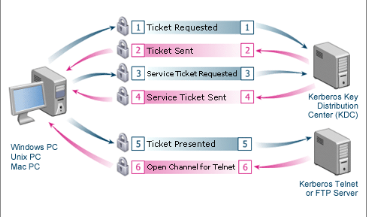
\includegraphics[width=0.9 \textwidth]{figuras/kerberos} 
   	\caption{Autenticação Kerberos \cite{KERBEROS}}
    \label{kerberos}
\end{figure}

%\pagebreak
 
%\section{NTP}

%Os servidores NTP permitem aos seus clientes a sincronização dos relógios de seus computadores e outros equipamentos de rede a partir de uma referência padrão de tempo aceita mundialmente, conhecida como UTC (\textit{Universal Time Coordinated}).\cite{RNP}

%\section{NTVFS}

%Sistema de arquivos que armazena os atributos do NTFS

\section{GSSAPI}

A GSSAPI é uma interface que permite aos desenvolvedores escreverem aplicações que aproveitam mecanismos de segurança tais como Kerberos, sem ter de programar explicitamente para qualquer mecanismo, ou seja, aplicações genéricas do ponto de vista de segurança. Programas que usam GSSAPI são, deste modo, altamente portáteis, não somente de uma plataforma para outra, mas de uma configuração de segurança a outra e de um protocolo de transporte a outro. A GSSAPI fornece vários níveis de proteção de dados, consistentes com os mecanismos de segurança subjacentes.\cite{HUGO}